\documentclass[letterpaper,11pt]{article}
\usepackage[letterpaper,top=3cm,bottom=3cm,left=3cm,right=3cm,marginparwidth=1.75cm]{geometry}



\usepackage[utf8]{inputenc} % allow utf-8 input
\usepackage[T1]{fontenc}    % use 8-bit T1 fonts
\usepackage{hyperref}       % hyperlinks
\usepackage{url}            % simple URL typesetting
\usepackage{booktabs}       % professional-quality tables
\usepackage{amsfonts}       % blackboard math symbols
\usepackage{nicefrac}       % compact symbols for 1/2, etc.
\usepackage{lipsum}
\usepackage{setspace}
\usepackage{comment}
\usepackage[ruled,vlined,boxed]{algorithm2e}
\usepackage{graphicx}



\doublespacing

\title{Multi-Armed Bandits with Variance considerations}


\begin{document}
\maketitle
\doublespacing

\begin{abstract}
Multi-armed bandit(MAB) methods are very effective in reducing the regret of the experimentation process especially in the presence of multiple policy levers. However, MAB algorithms only optimize the first moment(mean) of the outcome. In many clinical trials and public policy settings, variance estimation is as important as mean estimation, e.g., clinicians prefer lower variance treatments compared to higher ones even if the latter is slightly more effective. In this paper, we propose a vanilla hybrid algorithm that still minimizes regret compared to A/b testing but converges to true variance faster than the existing MAB algorithms. 
\end{abstract}

% keywords can be removed
{Keywords: Multi-armed bandit, A/B testing, sequential experimentation}

\section{Introduction}

A/B testing is an experimentation strategy to infer the effectiveness of an intervention compared to a baseline (control). A/B testing has been historically used in many scientific fields like Agriculture, Medicine, Social sciences and most recently it became popular in online experimentation. For a given tolerance of Type 1 and Type 2 errors, A/B testing is very effective in statistically rejecting a null hypothesis of the intervention (i.e. the intervention has no additional benefit compared to the baseline). During the experiment, subjects are allocated randomly to the baseline condition (control groups) and the intervention (treatment group). If the mean of the treatment outcomes is statistically different compared to the mean of control outcomes, we consider treatment to be effective.

Due to the proliferation of internet technologies, A/B testing is widely used on internet platforms (Microsoft ExP, Google Optimize, Optimizely, Monetate). A/B testing is used in variety of tasks, e.g., to test various design features of a website, test various marketing campaigns etc. While A/B testing is effective in this domain, it has many challenges. In the presence of multiple interventions, there is loss of utility (regret) in assigning subjects to sub-optimal conditions during experimentation process. Multi-armed bandit methods that use a combination of exploration and exploitation techniques are typically used to overcome this challenge. Allocation procedure in MAB methods is not random like in A/B testing. MAB's use dynamic allocation procedure based on outcome distribution at any given point of time. 

While Multi-armed bandits are very effective in online experimentation with large number of subjects, the algorithms only optimize for mean outcome. The allocation in MAB's is heavily skewed towards the treatment arm with higher mean irrespective of the variance. This is problematic if decision makers want to infer both mean and variance of treatment arms e.g., in clinical trials where a medicine that is slightly less effective but more accurate (low variance) is preferred to the one that is more effective on average but is less accurate (high variance), in public policy settings where one policy might be less effective compared to other but the outcomes have less variance.

For setting with multiple treatment arms with importance to inference of both mean and variance, we propose a hybrid algorithm (Hybrid-alg) and analyze its performance compared to A/B testing and MAB on various parameters like mean estimation, variance estimation, regret and convergence of variance. We find that while the Hybrid-alg's regret is comparable to that of MAB, it converges to true variance faster than a MAB. This is very useful in setting of clinical trials and public policy where the cost of treatment is very high and faster convergence to mean and variance could be traded for regret.



\begin{comment}
  
\end{comment}
 
 


\section{Overview}
\label{sec:headings}

The questions falls in the line of literature that is at the intersection of A/B testing, sequential experimentation and Multi-armed bandits. Below, we briefly review literature of these three topics and tie it with the question at hand. 


\subsection{A/B testing}
Experimental design is a statistical procedure for determining causality in the effect of a factor. The origin of experimental design can be traced to Fisher's Tea Tasting experiment. The field has been an active area of research is statistics since. And the field of experimental design has been of great interest to practitioners as well with applications in industrial process improvement, product design, clinical trials and more recently in the field of online testing. An experimental design can have multiple categorical and continuous factors that are varied carefully to estimate causally the effect of the factors or the lack of it on the outcome. For example, in a simple online experiment effect of placement of an ad on the top and bottom of the page can be tested by simultaneously testing effect of treatment on user clicks with different users. A single factor two level design is commonly referred to as A/B testing. Companies such as Google, Netflix use A/B testing extensively in applications such as website design, ad recommendation, movie recommendation among others. 

A typical A/B testing experiment has a treatment group who receive the treatment and control group who receive status quo. The effectiveness of experiments is determined by its ability to identify the active effects when present. In statistics literature failing to reject the Null hypothesis when alternative hypothesis is true is defined as Type II error. Type II error is not desired since the model fails to identify the active effect when it is present, consequently decreasing the utility of the experiment. Statistical Power is defined as the probability of rejecting the Null when the alternate hypothesis is true, the metric used to evaluate the effectiveness of the experiment. As the power increases the probability of Type II error decreases. Power is a function of the effect size of interest, variability in the outcome and the number of experimental runs. If the effect size is small or the outcome variance is low larger number of experimental runs is required to identify the effect. A desired power in statistical literature is 0.8.              
\subsection{Sequential Experimentation}
In classical experimental design the number of experimental runs and the factor levels for each runs are fixed in advance. Statistical Power is one criterion to determine the number of runs of the experiment to effectively reject the null hypothesis \cite{montgomery2017design}. In contrast sequential analysis refers to statistical theory and methods for experimentation in which the experimental values of each run depends on the observed past data \cite{johari2017peeking}. A sequential experiment terminates when a specified stopping criterion is met. If the stopping criterion is not met the experiment continues to sample an additional N+1 run. The key difference of sequential experimentation from classical experimentation is that the factor levels of each experimental run is adaptively chosen based on the observed values of the previous runs and the number of experimental runs need not be fixed in advance. Some applications of sequential analysis are industrial process control, clinical patient monitoring applications,  surveillance problems, medical and pharmaceutical applications among others.
\subsection{Multi-Armed Bandits}
Multi-armed bandit problems are sequential experimentation problems with an exploration–exploitation trade-off. The key decision in an armed bandit problem is the whether to stay with the highest payoff based on observed data and exploit the arm. Or explore other arms that might give higher payoffs in the future \cite{bubeck2012regret}. Bandit problems has been studied since the 1930s, exploration–exploitation trade-offs finds its application in several problem domains such as ad placement, website optimization, and packet routing \cite{bubeck2012regret}. 

A classical multi armed bandit setting is the slot machines at a casino. A gambler has n slot machines to choose from with unknown payoff and pulls the arm of slot machines until a fixed budget B is exhausted. The objective of the gambler is to maximize the total payoff obtained after a series of actions which exhausts the fixed budget. At each time step the gambler pulls an arm i and observes payoffs, and based on the past observations the gambler chooses the arm to pull in the next iteration. The above setting where the payoff is fixed and unknown is referred to as stochastic armed bandit. Another stream of literature is adversarial or non stochastic armed bandit formulation. In a non stochastic armed bandit setting the payoff is not fixed and the payoff is simultaneously chosen by the adversary upon observing or while the gambler pulls the arm. Commonly used stopping criterion in armed bandit setting is fixed budget as discussed earlier and fixed confidence setting where the experimentation stops when the confidence about the objective is above a persepcified threshold. An alternative formulation to exploitation vs exploration trade offs in armed bandit literature is the pure exploration formulation where the objective is to identify the best arm. In this formulation the gambler is asked to output a best arm with a prespecified confidence. 

A natural extension of armed bandits setting is to incorporate information about the environment into the decisions of the bandit algorithm. Such class of models are referred to as contextual bandits. Incorporating information on the context/environment is critical in settings such as online experiments. For example, if the decision is to display a news article for the user, the environment information could be user specific or article specific. User specific information is past historical activities, geographical location. While the environment information about the news article could be its recency, topic among others. Incorporating these decisions leads to better articles recommended to the user when compared with random selection of articles.


\section{Methodology}


The typical procedure of A/B is as follows. There is a baseline (control) condition. This is called placebo in clinical trials. In online experimentation setting, the control condition can be the existing state of a website. There is a treatment condition which is the intervention that needs to be tested (a new medicine or a new version of a website). An effect size (Cohen's D) is hypothesized and Type 1 and Type 2 error tolerances are fixed (typically type 1 error tolerance, alpha=0.05 and type 2 error rate 1-beta=0.8) in order to calculate sample size. These subjects are then randomly allocated to control and treatment conditions and outcomes are observed. A test statistic (e.g. t-test) is then used in order to infer if the treatment is statistically different from control. Even in the presence of multiple treatment, this is repeated for all treatment groups and the treatment with highest statistically significant effect size is chosen for final deployment. However, many treatments might be in effective and a lot of subjects are assigned to these groups as part of the random allocation leading to opportunity cost (regret).

Multi armed bandits overcome this by dynamic sequential allocation. Each allocation is done based on the outcomes of allocations so far. For example, in Upper confidence bound (UCB) algorithm, the upper confidence of each arm is calculated and a subject is allocated to the treatment with highest UCB, if the UCB reduces because of the allocation, the next subject is allocated to another arm with higher UCB (exploration). If the UCB still stays higher compared to other arms, then the next subject is allocated to the same arm (exploitation). In this case, it is possible that most subjects are allocated to the arm with higher mean and higher variance. This leads to lower allocation of subjects in all other treatment arms leading to insufficient inference of variance.  

We propose a vanilla hybrid algorithm that takes the best of both world's, i.e. minimize regret by dynamic allocation while also allocate enough to each arm to infer variance. We choose h\_alg between 0 and 1 which the fraction of times we make allocation using A/B testing rules and the rest of time we make allocation using any MAB. At each round, a coin is flipped with h\_alg probability and allocation rule is decided. We then run simulation by drawing outcomes from well known distributions in order to analyze how different algorithms perform at various metrics like mean outcome and variance error. 


\begin{algorithm}[]
\SetAlgoLined
\KwData{Control distribution, Treatment distribution, Total number of available subjects(N), alpha($\alpha$), power.}
Calculate n i.e. the number of subjects required to detect the effect size using power analysis \;
\For{i in n}{
Make treatment allocation \;
Observe outcome (draw from treatment distribution) \;
Make control allocation \;
Observe outcome (draw from control distribution) \;
}
\For{i in N-2n}{
\uIf {mean(control)<mean(treatment}{
Make treatment allocation \;
Observe outcome (draw from treatment distribution) \;
}
\Else{
Make control allocation \;
Observe outcome (draw from control distribution) \;
}
}
\caption{A/B testing Algorithm}

\end{algorithm}

\begin{algorithm}[]
\SetAlgoLined
\KwData{Control distribution, Treatment distribution, Total number of available subjects(N)}
\For{i in 2}{
Make treatment allocation \;
Observe outcome (draw from treatment distribution) \;
Make control allocation \;
Observe outcome (draw from control distribution) \;
}
\For{i in N-2}{
Find Upper Confidence bound for treatment \;
Find Upper Confidence bound for control \;

\uIf {UCB(control) < UCB(treatment}{
Make control allocation \;
Observe outcome (draw from control distribution) \;
}
\Else{
Make treatment allocation \;
Observe outcome (draw from treatment distribution) \;
}
}
\caption{UCB Algorithm}

\end{algorithm}


\begin{algorithm}[t]
\SetAlgoLined
\KwData{Control distribution, Treatment distribution, Total number of available subjects(N), Probability of A/B testing allocation (h\_alg) }

Draw from Bernoulli distribution with p=h\_alg \;

\uIf {0}{

Draw from Bernoulli distribution with p=0.5 \;

\uIf {0}{
Make control allocation \;
Observe outcome (draw from control distribution) \;
}
\Else{
Make treatment allocation \;
Observe outcome (draw from treatment distribution) \;

}}
\Else{
Find Upper Confidence bound for treatment \;
Find Upper Confidence bound for control \;

\uIf {UCB(control) < UCB(treatment}{
Make control allocation \;
Observe outcome (draw from control distribution) \;
}
\Else{
Make treatment allocation \;
Observe outcome (draw from treatment distribution) \;
}
}

\caption{Hybrid-alg Algorithm}

\end{algorithm}

\begin{figure}
  \centering
    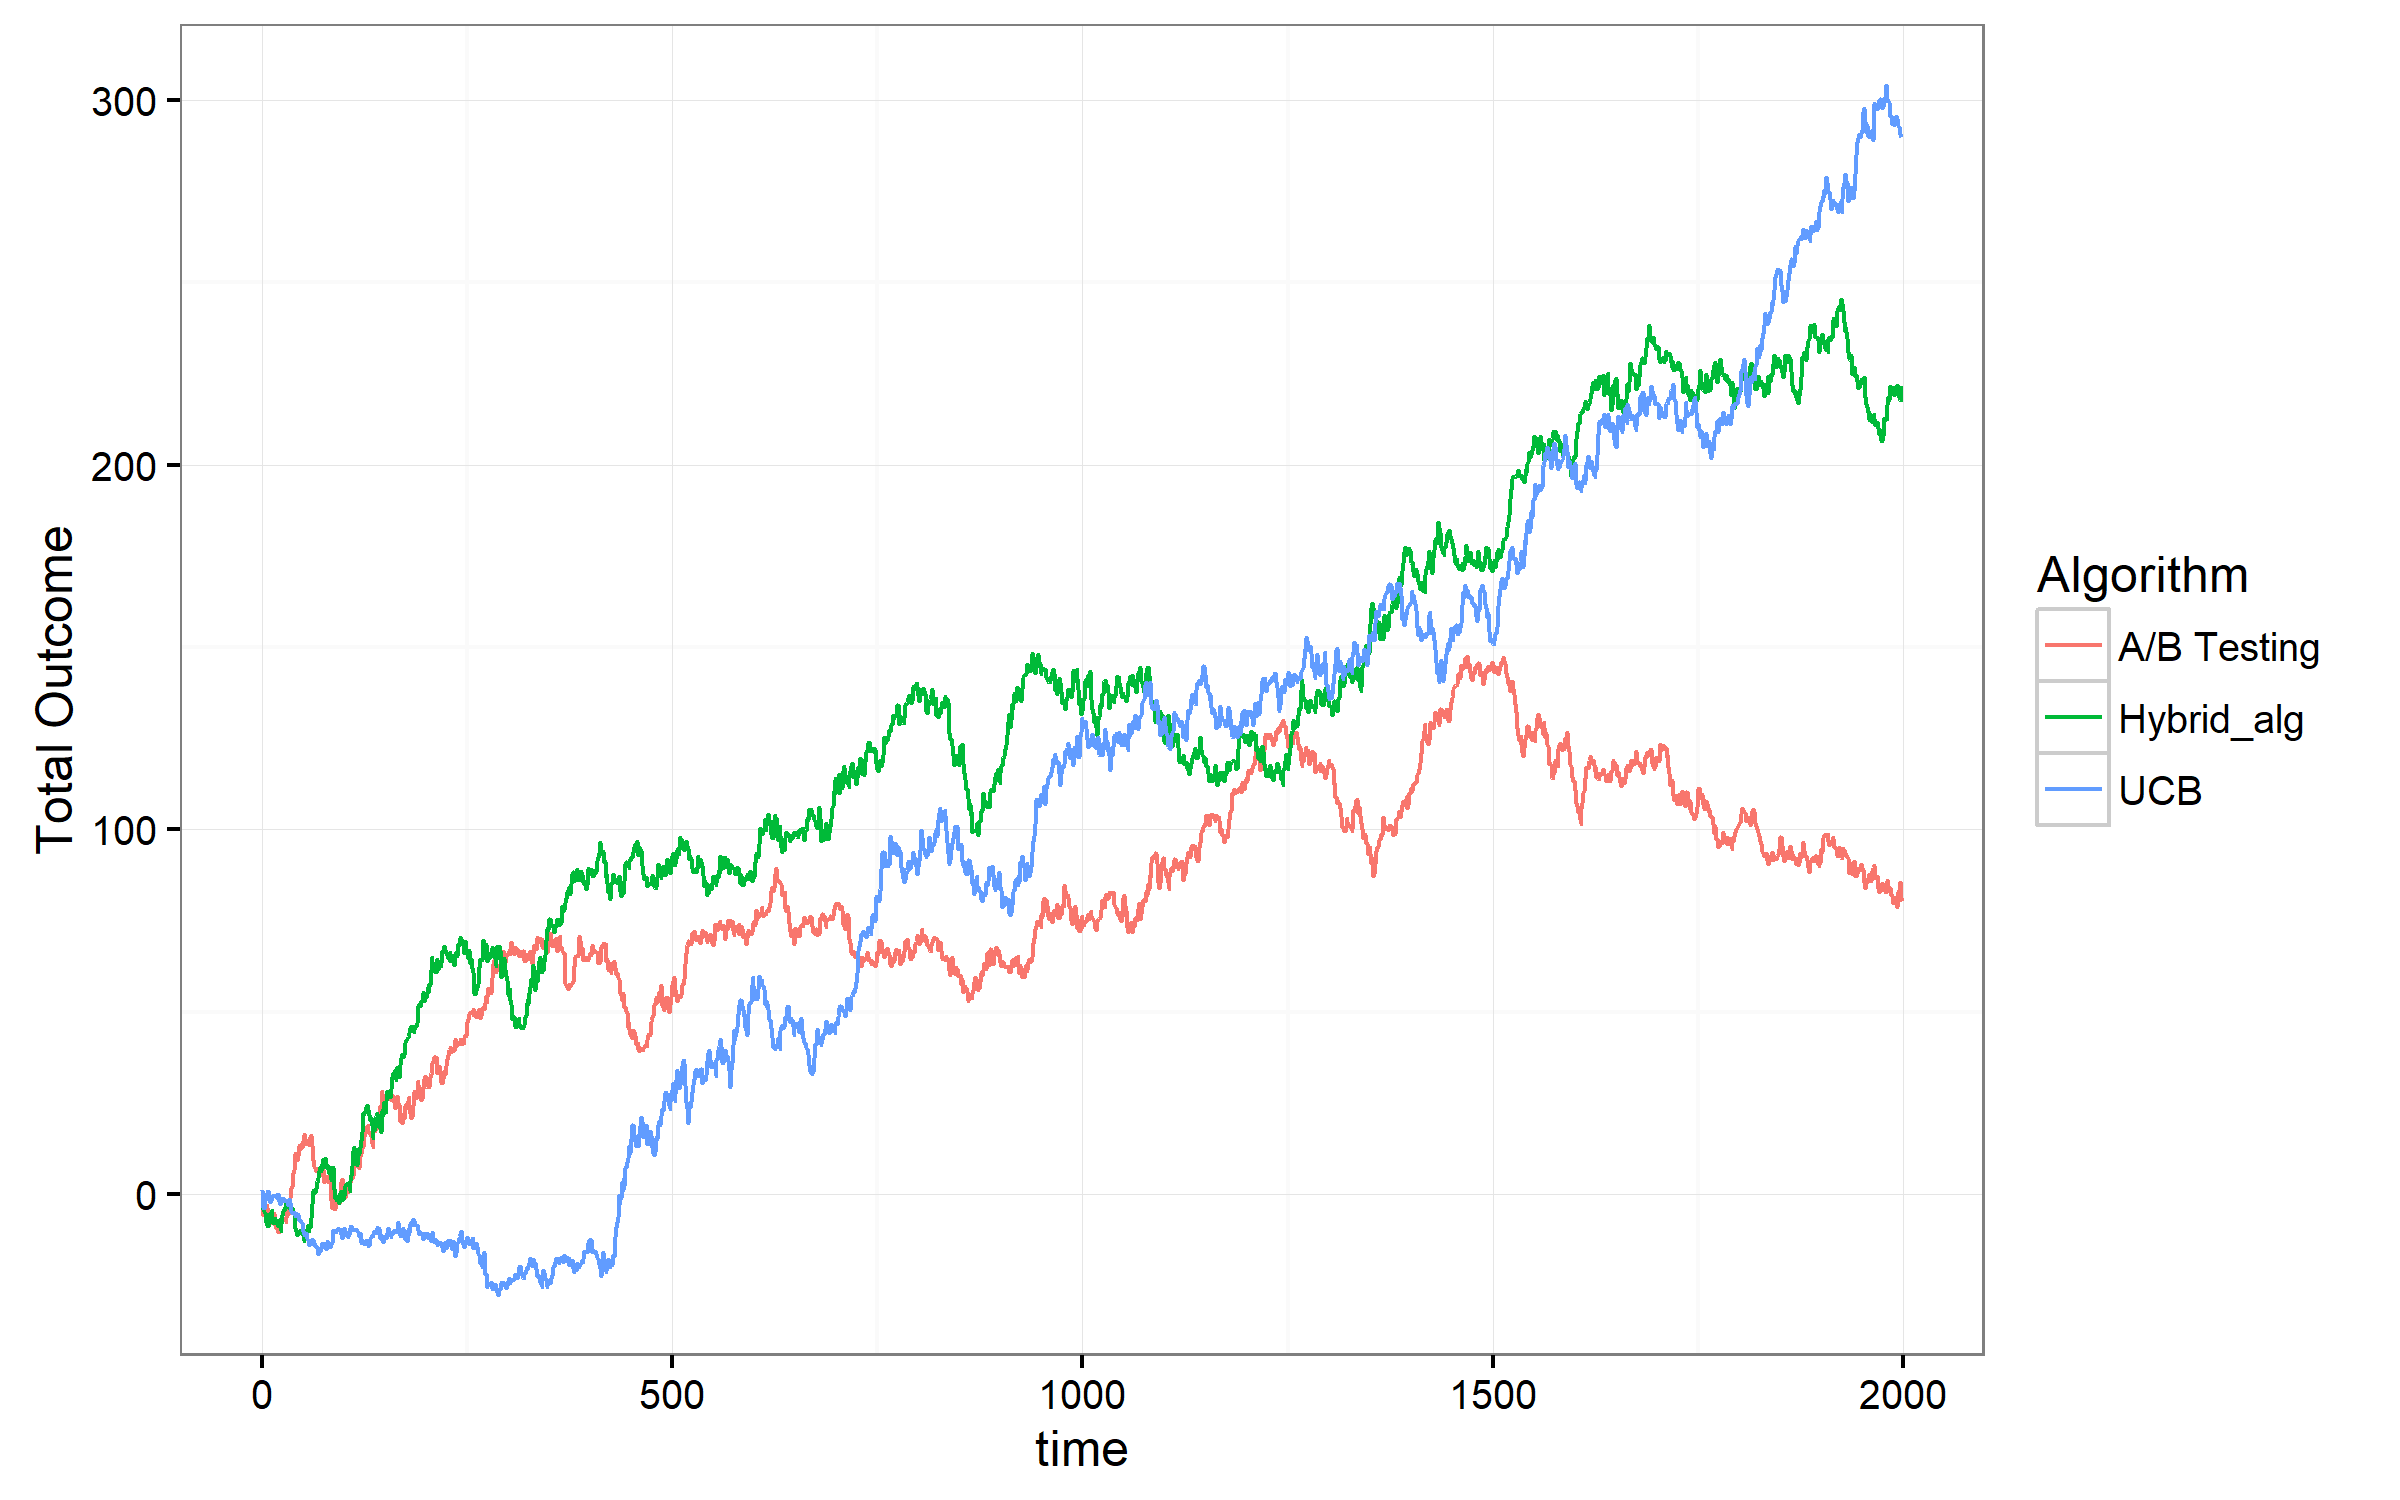
\includegraphics[width=\textwidth]{out.png}
      \caption{This figure shows the total realized outcome as per different algorithmic allocations}
    
\end{figure}


\section{Results}

We run simulation of A/B testing, UCB algorithm, and the Hybrid algorithm on control and treatment group outcomes which are drawn from $\mathcal{N}(0,1)$ and $\mathcal{N}(0.5,2)$ respectively. The variance of control group is 1 while the variance of treatment group is 4. As seen in Figure 1, the total outcome of UCB algorithm and Hybrid-alg are very similar and are significantly higher than that of A/B testing algorithm. This means that both are reducing the regret compared to A/B testing. Also in Figure 2 and Figure 3, we see that the estimation of variance for A/B testing is similar to that of Hybrid-alg for both control and treatment groups. But the variance estimate of UCB is very high compared to other algorithms. In conclusion, Hybrid-alg is getting the best of both world's i.e. lesser regret and accurate variance estimation. 



\begin{figure}
  \centering
    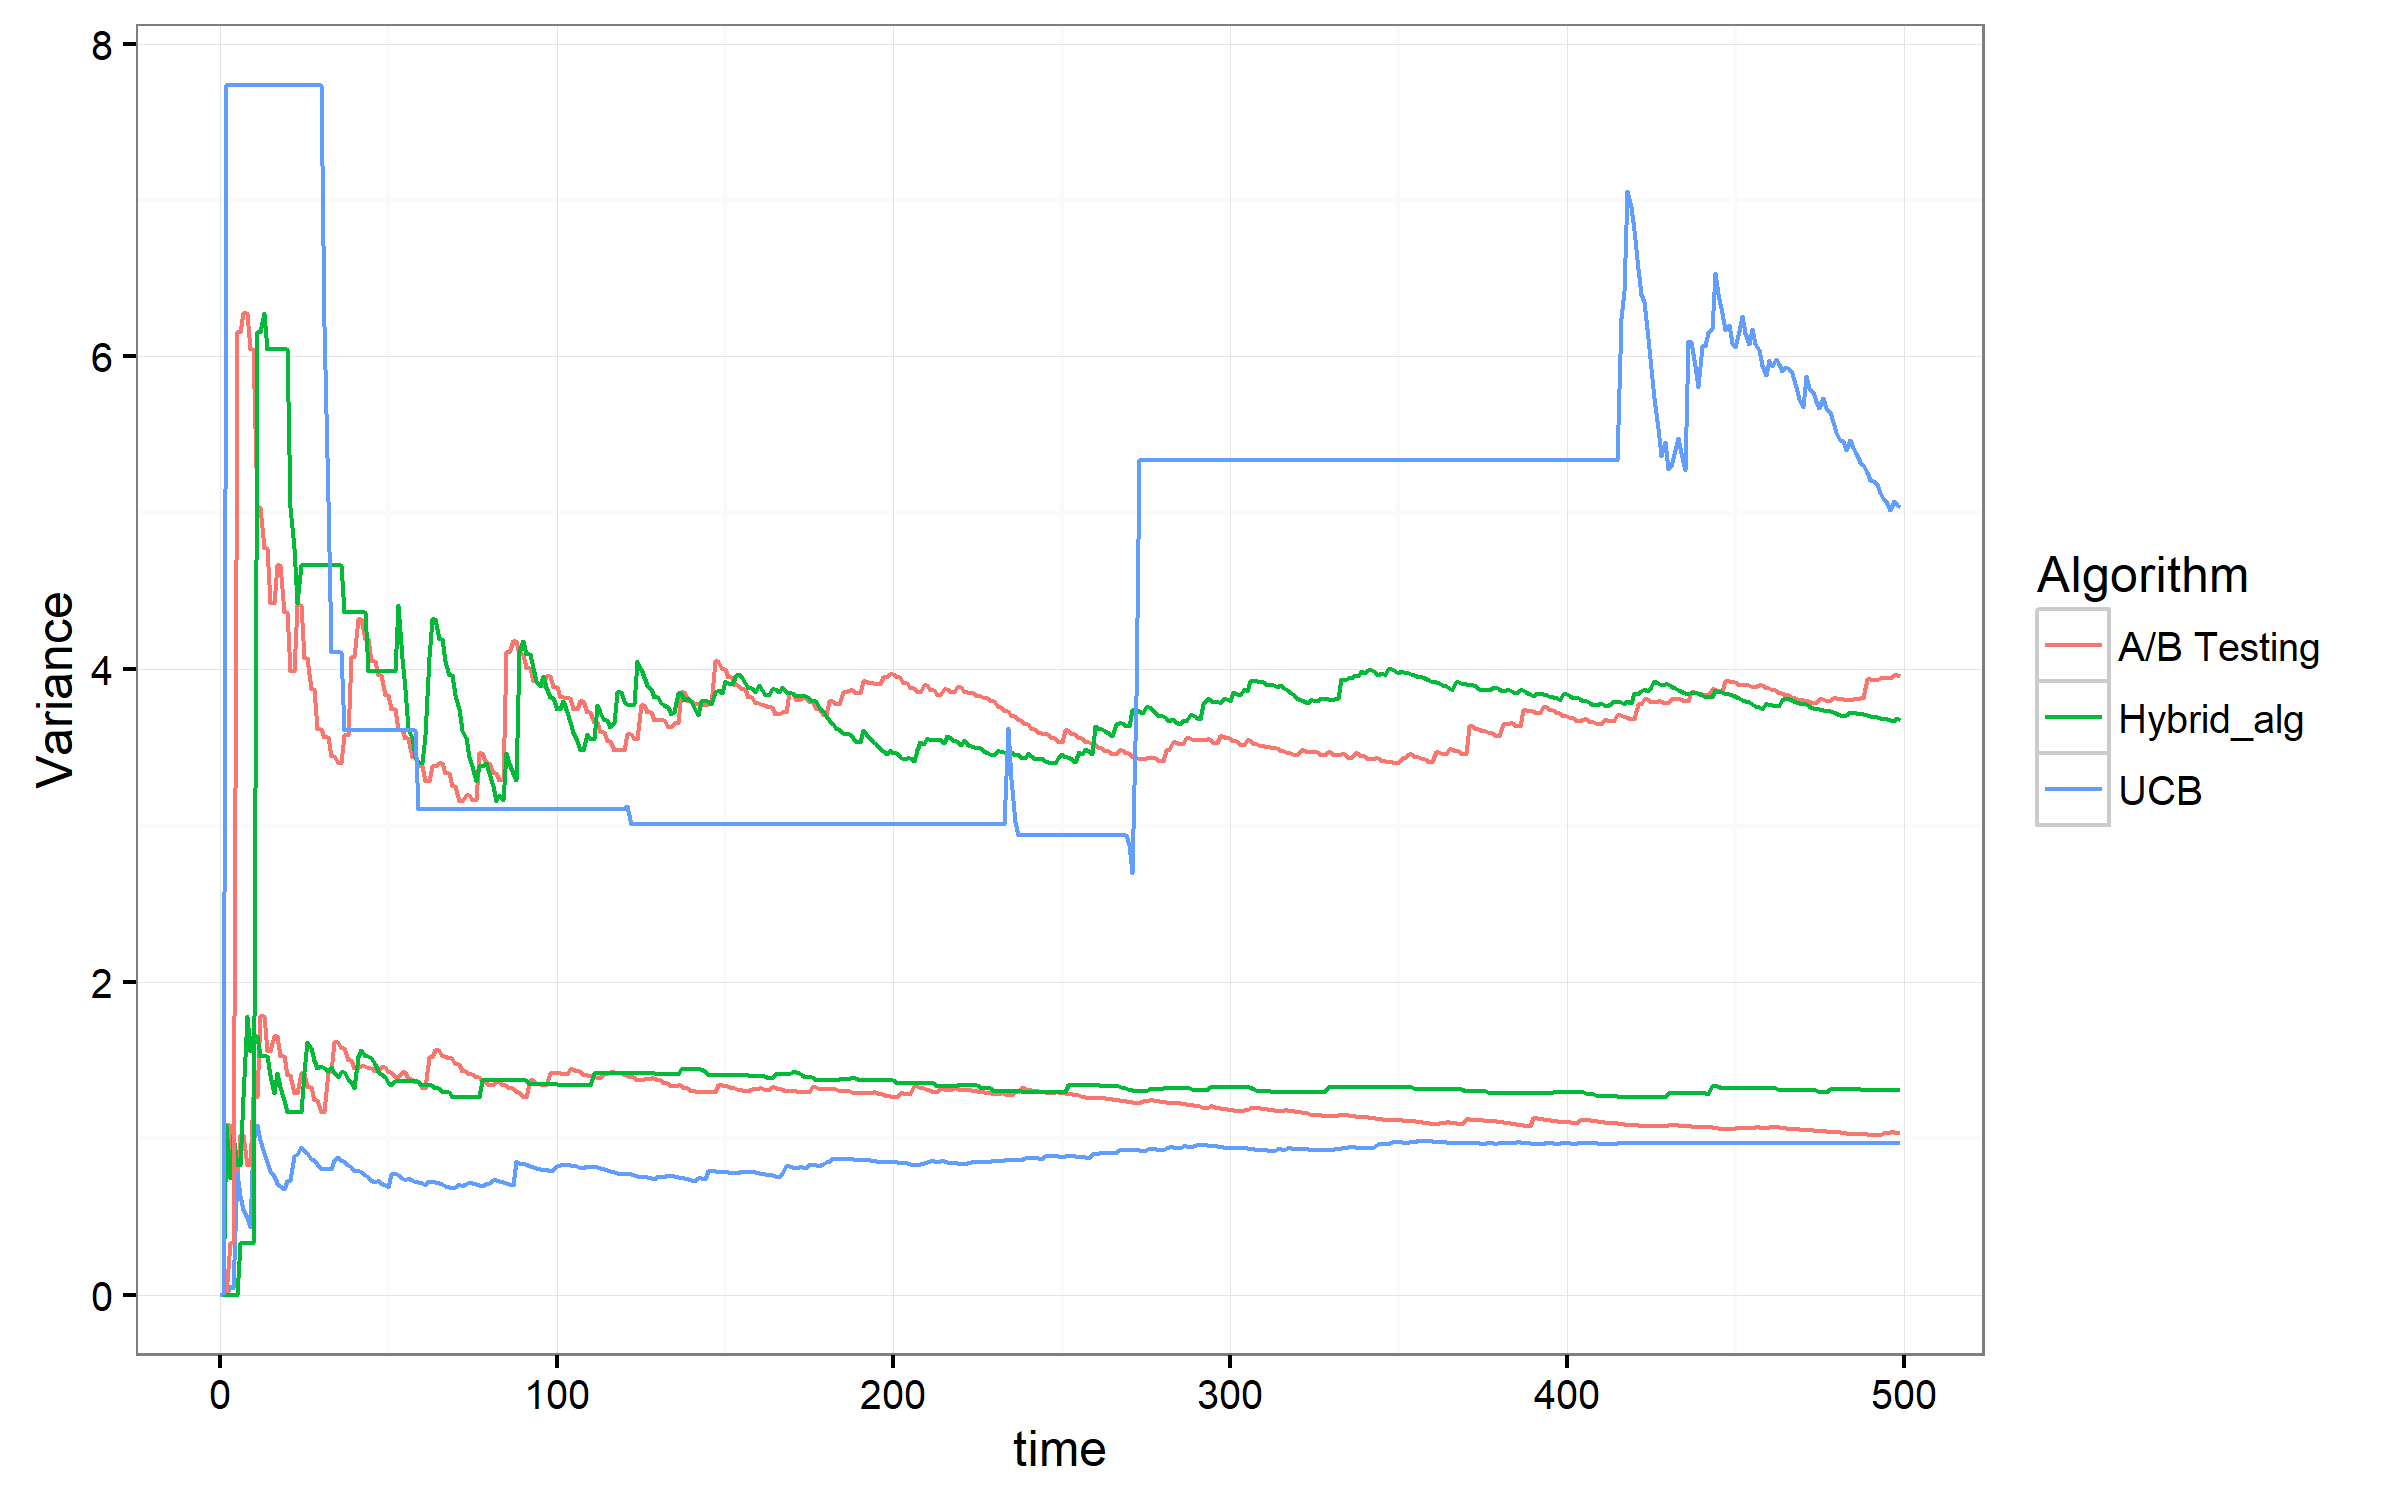
\includegraphics[width=\textwidth]{out_var.png}
      \caption{This figure shows the variance of outcomes of both treatment and control groups}
    
\end{figure}


\begin{figure}
  \centering
    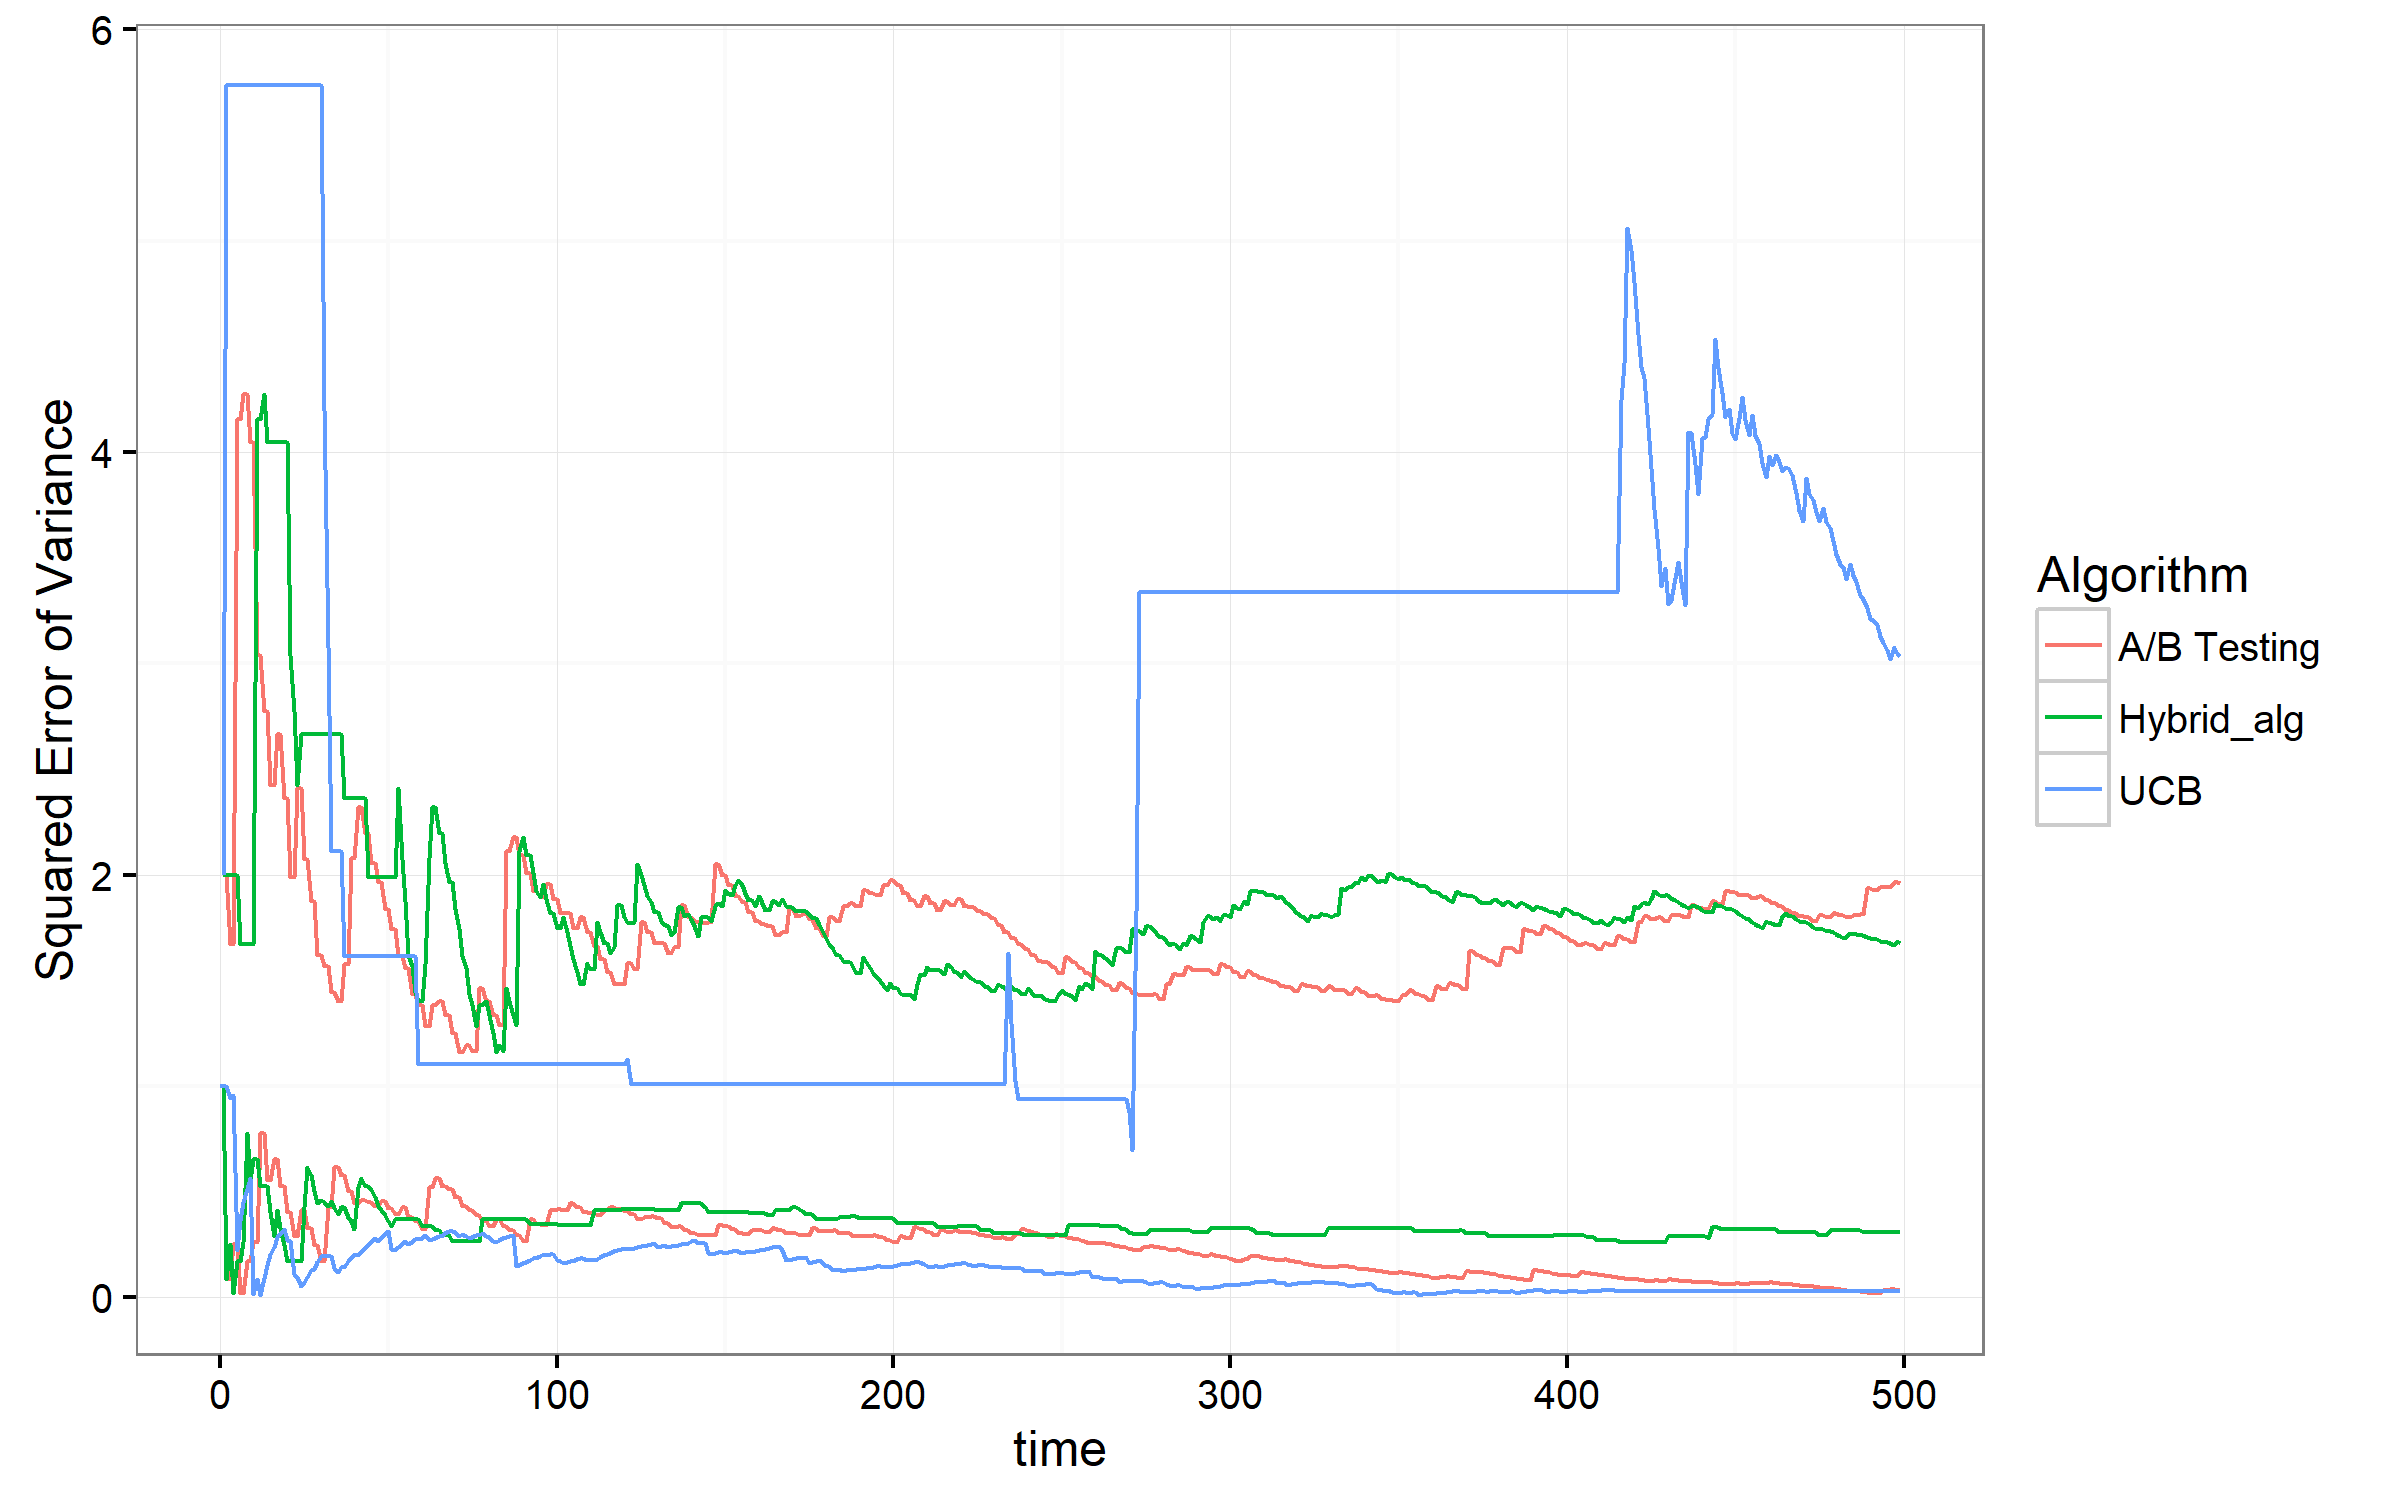
\includegraphics[width=\textwidth]{out_err.png}
      \caption{This figure shows squared error of estimated variance and the true variance}
    
\end{figure}



\section{Conclusion and Future Work}

In this paper, we propose a hybrid-alg, a vanilla hybrid algorithm that is a combination of A/B testing and Multi arm bandits and has the properties of both. It has regret comparable to that of UCB algorithm and variance estimate comparable to that of A/B testing. This is very useful in application related to clinical trials and public policy especially when there are multiple treatment arms and the number of available subjects are less or the cost of treatment is high. This algorithm makes the best worlds and is very efficient for practical purposes. \\

In future, we would want to do sensitivity analysis to see how the numbers vary for different MAB algorithms and different control/treatment distributions. We also recognize that this is a vanilla algorithm and an algorithm with dynamic variance inference and subsequent allocation would probably have better properties and might outperform the hybrid-alg. \\


\bibliography{references}{}
\bibliographystyle{plain}

\end{document}
